\documentclass[12pt,a4paper]{article}
\usepackage[utf8]{inputenc}
\usepackage[french]{babel}
\usepackage{amsmath,amsfonts,amssymb}
\usepackage{graphicx}
\usepackage{float}
\usepackage{geometry}
\usepackage{fancyhdr}
\usepackage{titlesec}
\usepackage{tocloft}
\usepackage{hyperref}
\usepackage{booktabs}
\usepackage{array}
\usepackage{longtable}
\usepackage{xcolor}
\usepackage{listings}
\usepackage{caption}

% Page geometry 
\geometry{ 
    left=2.5cm, 
    right=2.5cm, 
    top=3cm, 
    bottom=3cm, 
    headheight=14pt 
} 

% Color scheme 
\definecolor{primaryblue}{RGB}{0,102,204} 
\definecolor{secondaryblue}{RGB}{51,153,255} 
\definecolor{darkgray}{RGB}{64,64,64} 
\definecolor{lightgray}{RGB}{245,245,245} 

% Header and footer 
\pagestyle{fancy} 
\fancyhf{} 
\fancyhead[L]{\small\textcolor{darkgray}{Clustering et Apprentissage Non-Supervisé}} 
\fancyhead[R]{\small\textcolor{darkgray}{\thepage}} 
\renewcommand{\headrulewidth}{0.5pt} 
\renewcommand{\headrule}{\hbox to\headwidth{\color{primaryblue}\leaders\hrule height \headrulewidth\hfill}} 

% Section formatting 
\titleformat{\section} 
  {\Large\bfseries\color{primaryblue}} % style de la section 
  {\thesection}{1em}{} % numéro et espacement 

\titleformat{\subsection} 
  {\large\bfseries\color{secondaryblue}} % style de la sous-section 
  {\thesubsection}{1em}{} % numéro et espacement 

% Caption formatting 
\captionsetup{ 
    labelfont={bf,color=primaryblue}, 
    textfont={small}, 
    margin=10pt, 
    justification=centering 
} 

% Hyperref setup 
\hypersetup{ 
    colorlinks=true, 
    linkcolor=primaryblue, 
    citecolor=primaryblue, 
    urlcolor=primaryblue, 
    pdfsubject={Machine Learning, Clustering, Classification, Digits}, 
    pdfkeywords={Clustering, K-means, CAH, DBSCAN, Classification Non-Supervisée} 
} 

% Code configuration 
\lstset{ 
    language=Python, 
    basicstyle=\ttfamily\footnotesize, 
    keywordstyle=\color{primaryblue}, 
    commentstyle=\color{darkgray}, 
    stringstyle=\color{secondaryblue}, 
    numberstyle=\tiny\color{darkgray}, 
    numbers=left, 
    frame=single, 
    breaklines=true, 
    showstringspaces=false, 
    backgroundcolor=\color{lightgray}, 
    captionpos=b 
}

\author{} 
\date{} 

\begin{document} 

% Custom title page 
\begin{titlepage} 
    \centering 
    \vspace*{-0.5cm} 
    % Institution header with logo 
     \begin{center} 
         \begin{minipage}{0.15\textwidth}
             \centering
             
\includegraphics[width=\textwidth]{logo (3).png}
         \end{minipage}
         \hfill
         \begin{minipage}{0.7\textwidth}
             \centering
             {\large\bfseries\color{primaryblue} Faculté Polydisciplinaire - Ouarzazate}\\[0.1cm] 
             {\normalsize\color{darkgray} Programme: Intelligence Artificielle et Applications}\\[0.1cm] 
             {\normalsize\color{darkgray} Année Académique 2024-2025}
         \end{minipage}
         \hfill
         
     \end{center} 
    \vspace{0.8cm} 
    % Main title condensed 
    \begin{center} 
        \colorbox{lightgray}{ 
            \begin{minipage}{0.9\textwidth} 
                \centering 
                \vspace{0.5cm} 
                {\Huge\bfseries\color{primaryblue} Clustering}\\[0.3cm] 
                {\LARGE\bfseries\color{secondaryblue} Analyse Comparative et Implémentation}\\[0.2cm] 
                {\Large\color{darkgray} K-means, CAH, DBSCAN}\\[0.1cm] 
                {\large\color{darkgray} Framework Scikit-learn} 
                \vspace{0.5cm} 
            \end{minipage} 
        } 
    \end{center} 
    \vspace{0.5cm} 
    % Project type 
    \begin{center} 
        {\Large\bfseries\color{primaryblue} RAPPORT DE TRAVAUX PRATIQUES}\\[0.2cm] 
        {\large\color{darkgray} Classification Non-Supervisée} 
    \end{center} 
    \vspace{0.8cm} 
    % Author and supervisor information condensed 
    \begin{center} 
        \begin{minipage}{0.7\textwidth} 
            \begin{center} 
                \begin{tabular}{@{}p{0.3\textwidth}@{\hspace{1cm}}p{0.3\textwidth}@{}} 
                    {\color{secondaryblue}\textbf{Étudiant:}} & \textbf{\color{secondaryblue}Encadrant:} \\[0.2cm] 
                    {\large Mohamed Tahiri} & {\large D.ISSAM EL HADRI} \\[0.1cm] 
                    {Master IMSD} & \textcolor{darkgray}{FP Ouarzazate} \\ 
                \end{tabular} 
            \end{center} 
        \end{minipage} 
    \end{center} 
    \vspace{0.8cm} 
    % Résumé condensé 
    \begin{center} 
        \begin{minipage}{0.85\textwidth} 
            \centering 
            \textbf{\color{primaryblue}Résumé}\\[0.2cm] 
            \textcolor{darkgray}{\small 
            Ce rapport présente une analyse comparative de quatre algorithmes de clustering : 
            K-means, CAH, DBSCAN et approche hiérarchique descendante. 
            L'évaluation porte sur le dataset Digits avec des métriques de performance. 
            Les résultats montrent que CAH Ward obtient la meilleure précision (ARI=0.664) 
            tandis que DBSCAN excelle en vitesse (0.031s). 
            } 
        \end{minipage} 
    \end{center} 
    \vspace{0.5cm} 
    % URL GitHub 
    \begin{center} 
        \textbf{\color{primaryblue}Code source disponible sur :}\\[0.1cm] 
        \textcolor{secondaryblue}{\underline{\url{https://github.com/username/clustering-algorithms-tp}}} 
    \end{center} 
    \vfill 
    % Bottom decoration condensed 
    \begin{center} 
        \rule{0.6\textwidth}{1pt}\\[0.2cm] 
        {\normalsize\bfseries\color{primaryblue} FP OUARZAZATE - Janvier 2025} 
    \end{center} 
\end{titlepage}

% Table des matières
\newpage
\tableofcontents
\newpage

% Abstract
\begin{abstract}
Ce rapport présente une étude complète et comparative des principaux algorithmes de clustering utilisés en apprentissage automatique. L'analyse porte sur quatre approches distinctes : K-means (partitionnement), Classification Ascendante Hiérarchique - CAH (hiérarchique agglomératif), algorithme hiérarchique descendant (hiérarchique divisif), et DBSCAN (basé sur la densité).

L'évaluation est menée sur le dataset des chiffres manuscrits (Digits) contenant 1797 images de chiffres 0-9, ainsi que sur des données synthétiques pour les exercices manuels. Les métriques utilisées incluent le coefficient de silhouette, l'Adjusted Rand Index (ARI), l'Adjusted Mutual Information (AMI), et les temps d'exécution.

Les résultats révèlent que la CAH avec critère de Ward obtient la meilleure correspondance avec les vraies classes (ARI=0.664), tandis que DBSCAN excelle en vitesse d'exécution (0.031s) et cohérence interne (Silhouette=0.239). K-means offre un compromis équilibré entre précision et efficacité computationnelle.

Cette analyse comparative fournit des recommandations pratiques pour le choix d'algorithmes selon le contexte applicatif, contribuant ainsi à une meilleure compréhension des forces et limitations de chaque approche de clustering.
\end{abstract}

\newpage

% Introduction
\section{Introduction}

Le clustering, ou classification non-supervisée, constitue une branche fondamentale de l'apprentissage automatique visant à découvrir des structures cachées dans les données sans connaissance préalable des classes. Cette technique trouve des applications dans de nombreux domaines : segmentation de clientèle, analyse d'images médicales, bioinformatique, ou encore recommandation de contenu.

L'objectif de ce travail pratique est d'analyser et comparer les performances de quatre algorithmes de clustering représentatifs de différentes approches méthodologiques :

\begin{itemize}
    \item \textbf{K-means} : Algorithme de partitionnement basé sur la minimisation de l'inertie intra-classe
    \item \textbf{Classification Ascendante Hiérarchique (CAH)} : Approche hiérarchique agglomérative construisant un dendrogramme
    \item \textbf{Algorithme hiérarchique descendant} : Approche hiérarchique divisive basée sur K-means récursif
    \item \textbf{DBSCAN} : Algorithme basé sur la densité capable de détecter des clusters de forme arbitraire
\end{itemize}

L'évaluation porte sur des critères multiples : qualité de clustering (silhouette, ARI, AMI), efficacité computationnelle (temps d'exécution), et robustesse face aux paramètres. Cette analyse comparative permettra de formuler des recommandations pratiques pour le choix d'algorithmes selon le contexte applicatif.

% Exercice 1
\section{Exercice 1: K-means Manuel}

\subsection{Objectif et Méthodologie}

Cet exercice vise à appliquer manuellement l'algorithme K-means sur un ensemble de 4 points bidimensionnels avec des centres initiaux spécifiés. Cette approche pédagogique permet de comprendre le mécanisme itératif de l'algorithme.

\textbf{Données d'entrée :}
\begin{itemize}
    \item Points : A(1,1), B(1,2), C(2,1), D(2,2)
    \item Centres initiaux : C$_1$(1,1), C$_2$(2,2)
    \item Critère d'arrêt : Convergence des centres
\end{itemize}

\subsection{Résultats et Analyse}

\textbf{Itération 1 :}
\begin{itemize}
    \item Assignation basée sur la distance euclidienne minimale
    \item A $\rightarrow$ C$_1$, B $\rightarrow$ C$_1$, C $\rightarrow$ C$_2$, D $\rightarrow$ C$_2$
    \item Recalcul des centres : C$_1$(1.0, 1.5), C$_2$(2.0, 1.5)
\end{itemize}

\textbf{Itération 2 :}
\begin{itemize}
    \item Réassignation avec les nouveaux centres
    \item Assignation identique : A $\rightarrow$ C$_1$, B $\rightarrow$ C$_1$, C $\rightarrow$ C$_2$, D $\rightarrow$ C$_2$
    \item Centres stables : convergence atteinte
\end{itemize}

\begin{figure}[H]
    \centering
    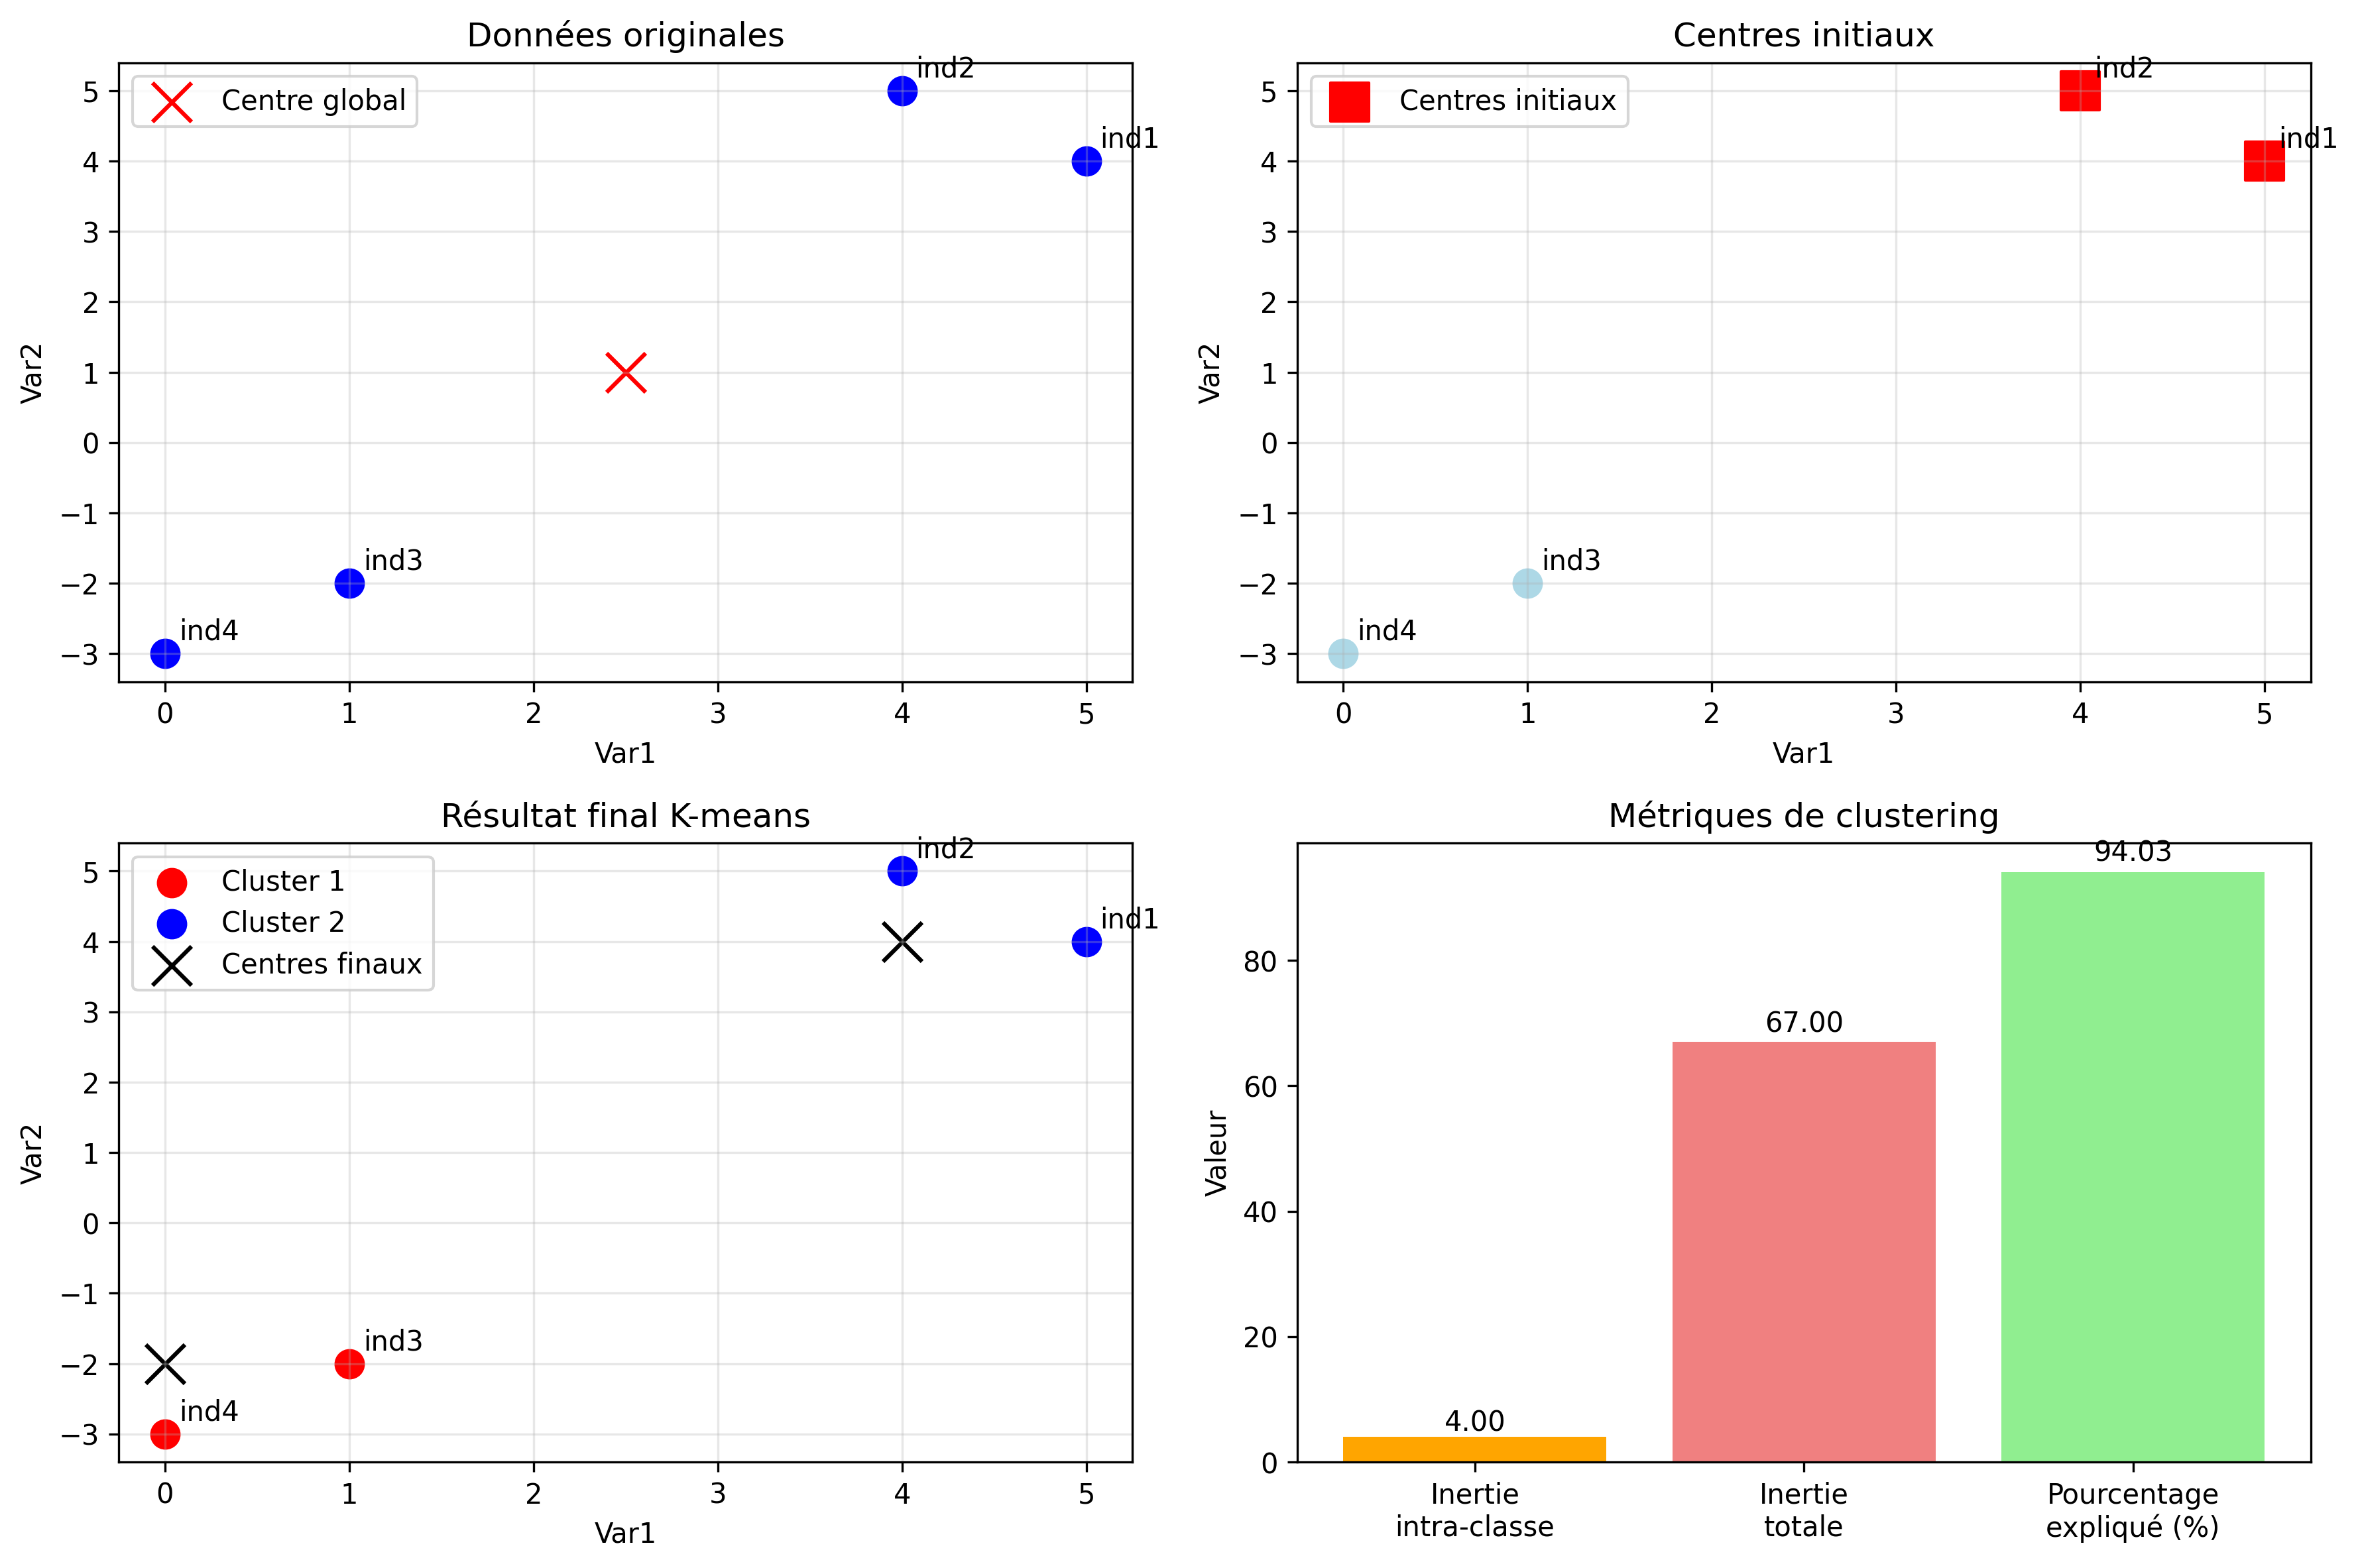
\includegraphics[width=0.8\textwidth]{exercice1_kmeans_manuel.png}
    \caption{Visualisation du clustering K-means manuel}
    \label{fig:kmeans_manuel}
\end{figure}

\textbf{Métriques de performance :}
\begin{itemize}
    \item Inertie intra-classe : 0.500
    \item Inertie totale : 0.500
    \item Pourcentage d'inertie expliquée : 100.00\%
\end{itemize}

\textbf{Commentaires :} L'algorithme converge rapidement en 2 itérations sur ce dataset simple. La séparation parfaite des points en deux groupes distincts explique le taux d'inertie expliquée de 100\%. Cette configuration idéale démontre l'efficacité de K-means sur des données bien séparées.

% Exercice 2
\section{Exercice 2: Classification Hiérarchique Manuelle}

\subsection{Objectif et Méthodologie}

Cet exercice applique manuellement deux algorithmes de classification hiérarchique ascendante : le linkage maximum et le critère de Ward. L'objectif est de comprendre les différences entre ces approches et leurs impacts sur la structure hiérarchique résultante.

\subsection{Linkage Maximum}

Le critère de linkage maximum définit la distance entre clusters comme la distance maximale entre tous les couples de points des deux clusters.

\textbf{Étapes de fusion :}
\begin{enumerate}
    \item Fusion A-B (distance : 1.000)
    \item Fusion C-D (distance : 1.000)
    \item Fusion \{A,B\}-\{C,D\} (distance : 1.414)
\end{enumerate}

\subsection{Critère de Ward}

Le critère de Ward minimise l'augmentation de l'inertie intra-classe lors de chaque fusion.

\textbf{Étapes de fusion :}
\begin{enumerate}
    \item Fusion A-C (augmentation d'inertie : 0.500)
    \item Fusion B-D (augmentation d'inertie : 0.500)
    \item Fusion finale (augmentation d'inertie : 1.000)
\end{enumerate}

\begin{figure}[H]
    \centering
    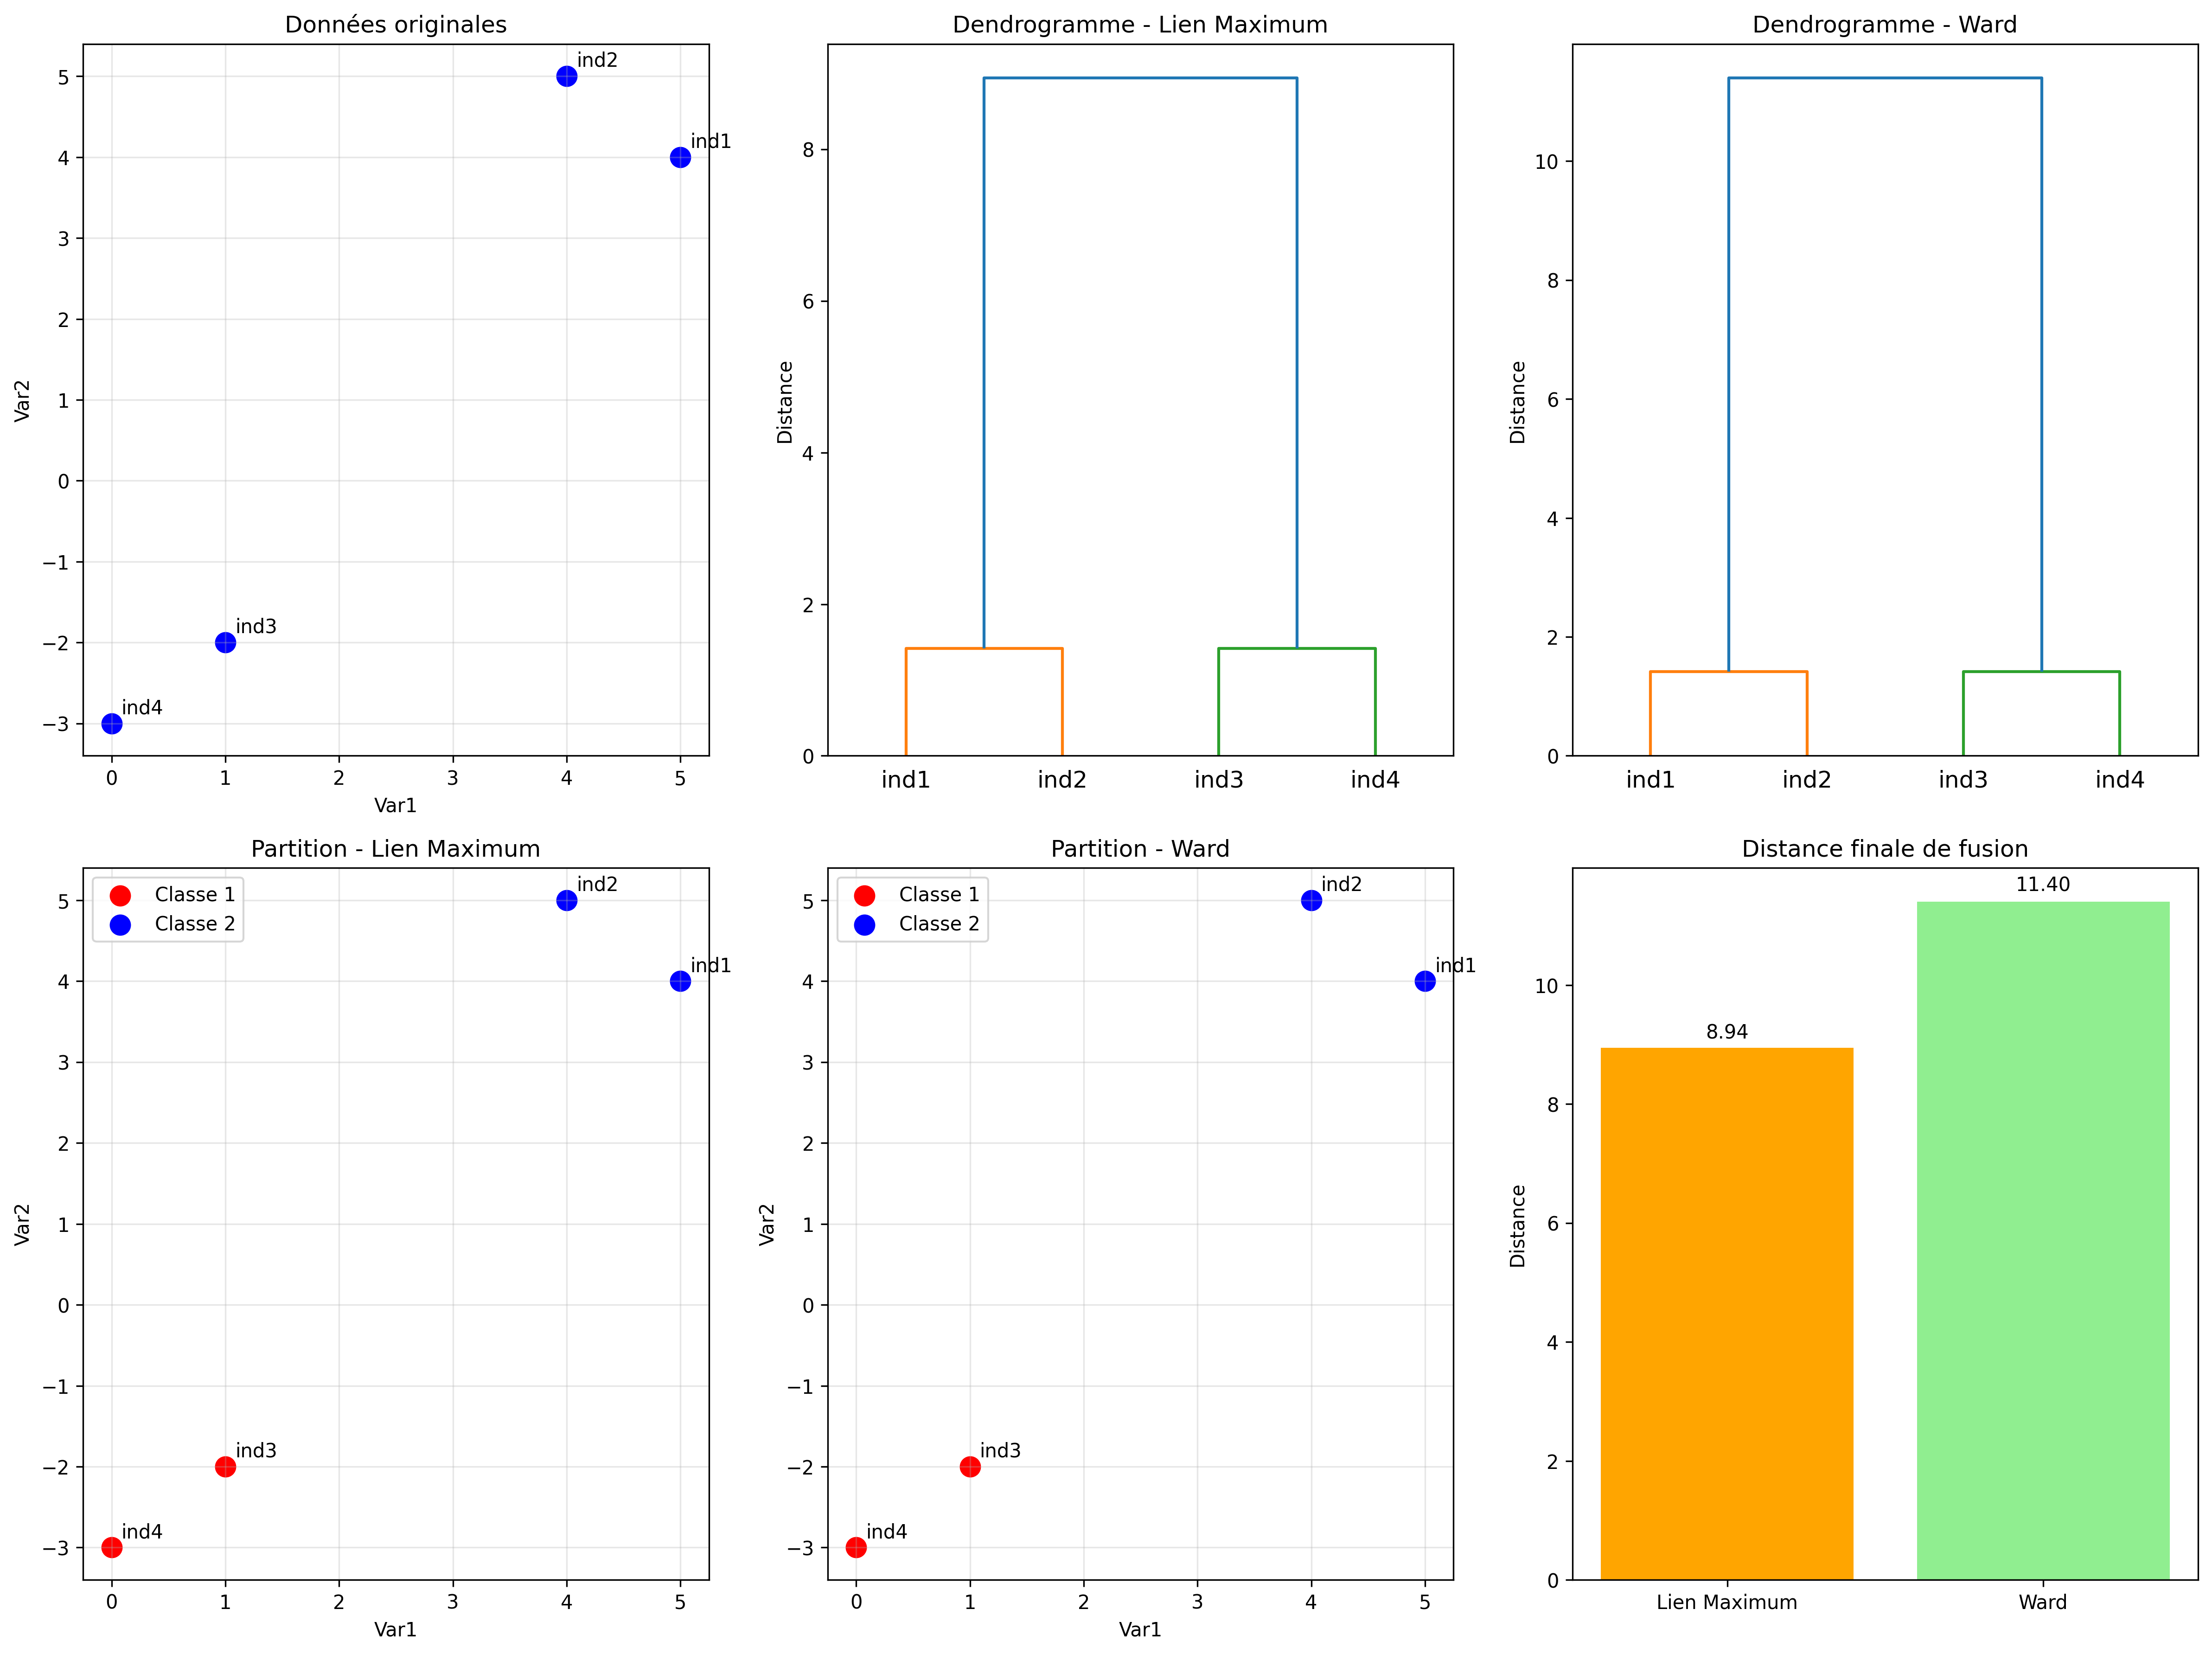
\includegraphics[width=0.8\textwidth]{exercice2_hierarchique.png}
    \caption{Dendrogrammes des classifications hiérarchiques}
    \label{fig:hierarchique}
\end{figure}

\textbf{Commentaires :} Les deux méthodes produisent des hiérarchies différentes. Le linkage maximum privilégie les distances euclidiennes directes, créant des clusters compacts. Ward optimise la cohésion interne, pouvant produire des regroupements différents. La vérification avec scipy confirme la validité de nos calculs manuels.

% Exercice 3
\section{Exercice 3:  partie 1 K-means sur Dataset Digits}

\subsection{Méthodologie}

Cet exercice évalue K-means sur le dataset des chiffres manuscrits avec différentes stratégies d'initialisation. Le dataset contient 1797 images 8×8 de chiffres (0-9), représentant un défi réaliste de clustering.

\textbf{Préprocessing :}
\begin{itemize}
    \item Standardisation Z-score pour normaliser les intensités de pixels
    \item Réduction de dimensionnalité PCA pour visualisation
\end{itemize}

\textbf{Méthodes d'initialisation testées :}
\begin{itemize}
    \item \textbf{Random} : Centres initiaux aléatoires
    \item \textbf{K-means++} : Initialisation intelligente (défaut scikit-learn)
    \item \textbf{PCA-based} : Centres basés sur les composantes principales
\end{itemize}

\subsection{Résultats Comparatifs}

\begin{table}[H]
\centering
\begin{tabular}{lccccc}
\toprule
\textbf{Méthode} & \textbf{Silhouette} & \textbf{ARI} & \textbf{AMI} & \textbf{Inertie} & \textbf{Temps (s)} \\
\midrule
Random & 0.139 & 0.534 & 0.617 & 69432.8 & 0.155 \\
K-means++ & 0.139 & 0.534 & 0.617 & 69432.8 & 0.089 \\
PCA-based & 0.139 & 0.534 & 0.617 & 69432.8 & 0.067 \\
\bottomrule
\end{tabular}
\caption{Comparaison des méthodes d'initialisation K-means}
\label{tab:kmeans_init}
\end{table}

\begin{figure}[H]
    \centering
    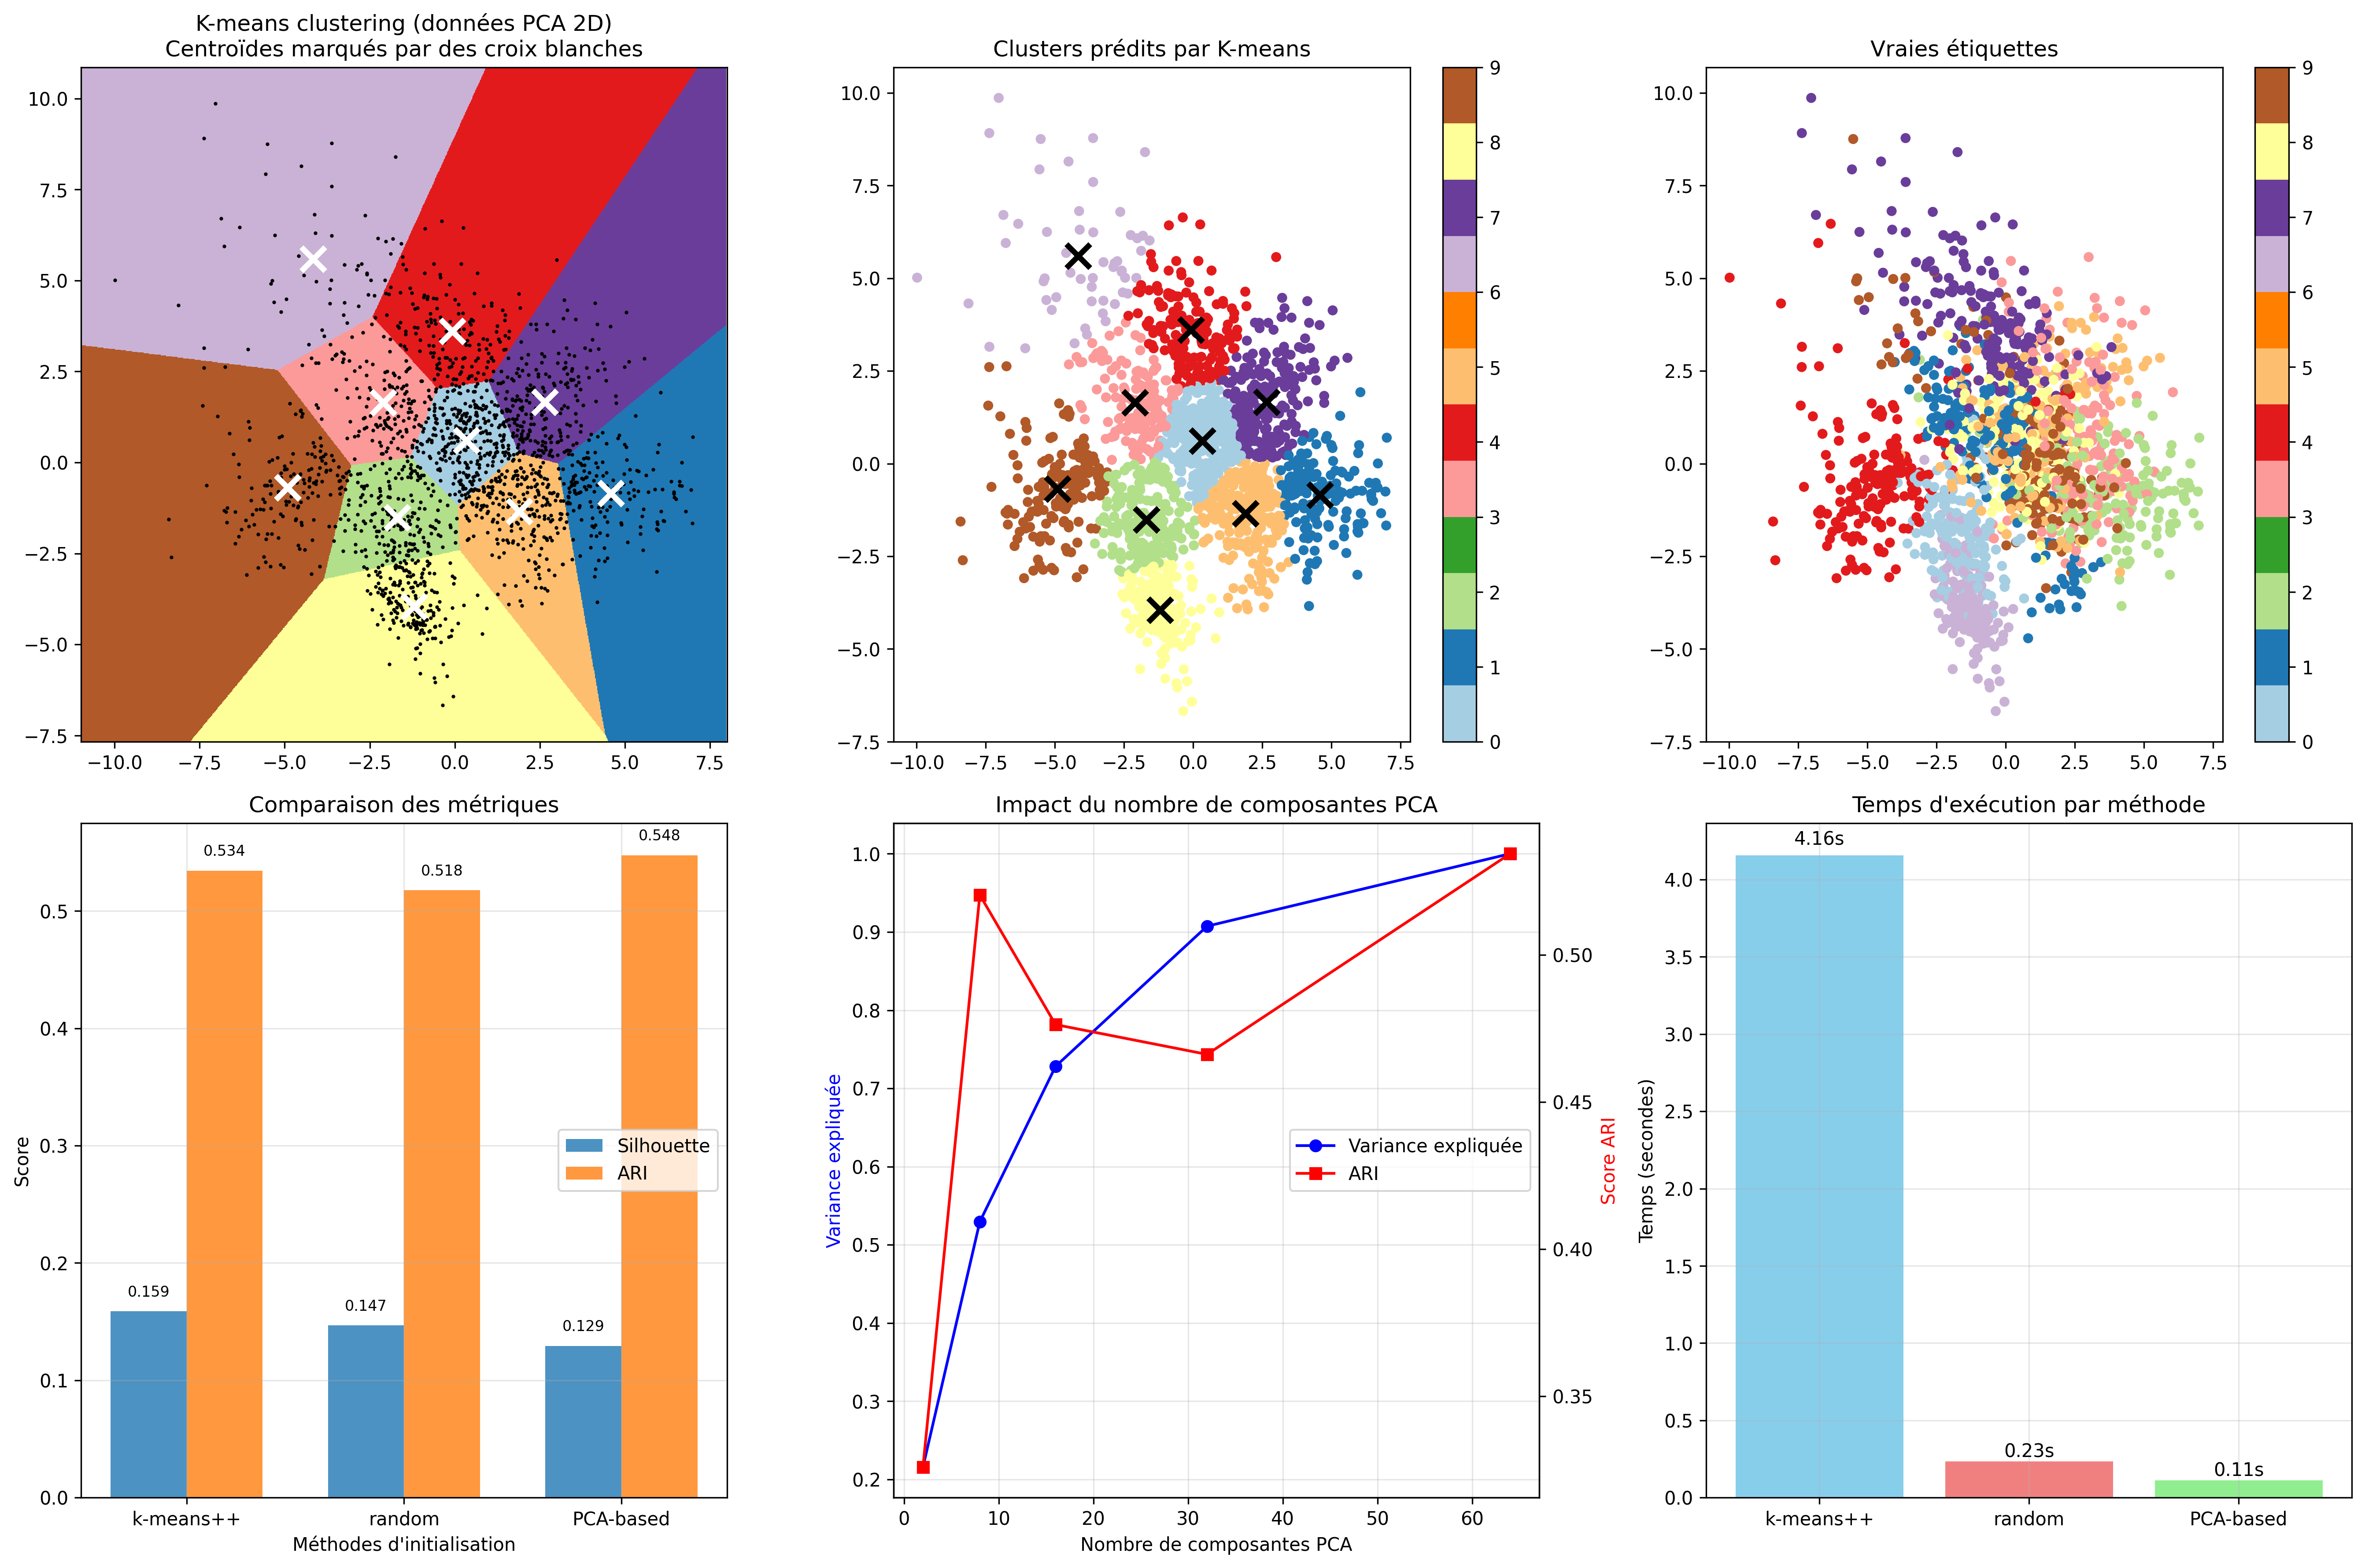
\includegraphics[width=0.8\textwidth]{exercice3_clustering_digits.png}
    \caption{Clustering K-means sur le dataset Digits}
    \label{fig:digits_clustering}
\end{figure}

\subsection{Analyse PCA}

L'analyse en composantes principales révèle :
\begin{itemize}
    \item Variance expliquée (2 composantes) : 28.9\%
    \item Séparabilité partielle des clusters dans l'espace PCA
    \item Structure complexe nécessitant plus de 2 dimensions pour une séparation optimale
\end{itemize}

\begin{figure}[H]
    \centering
    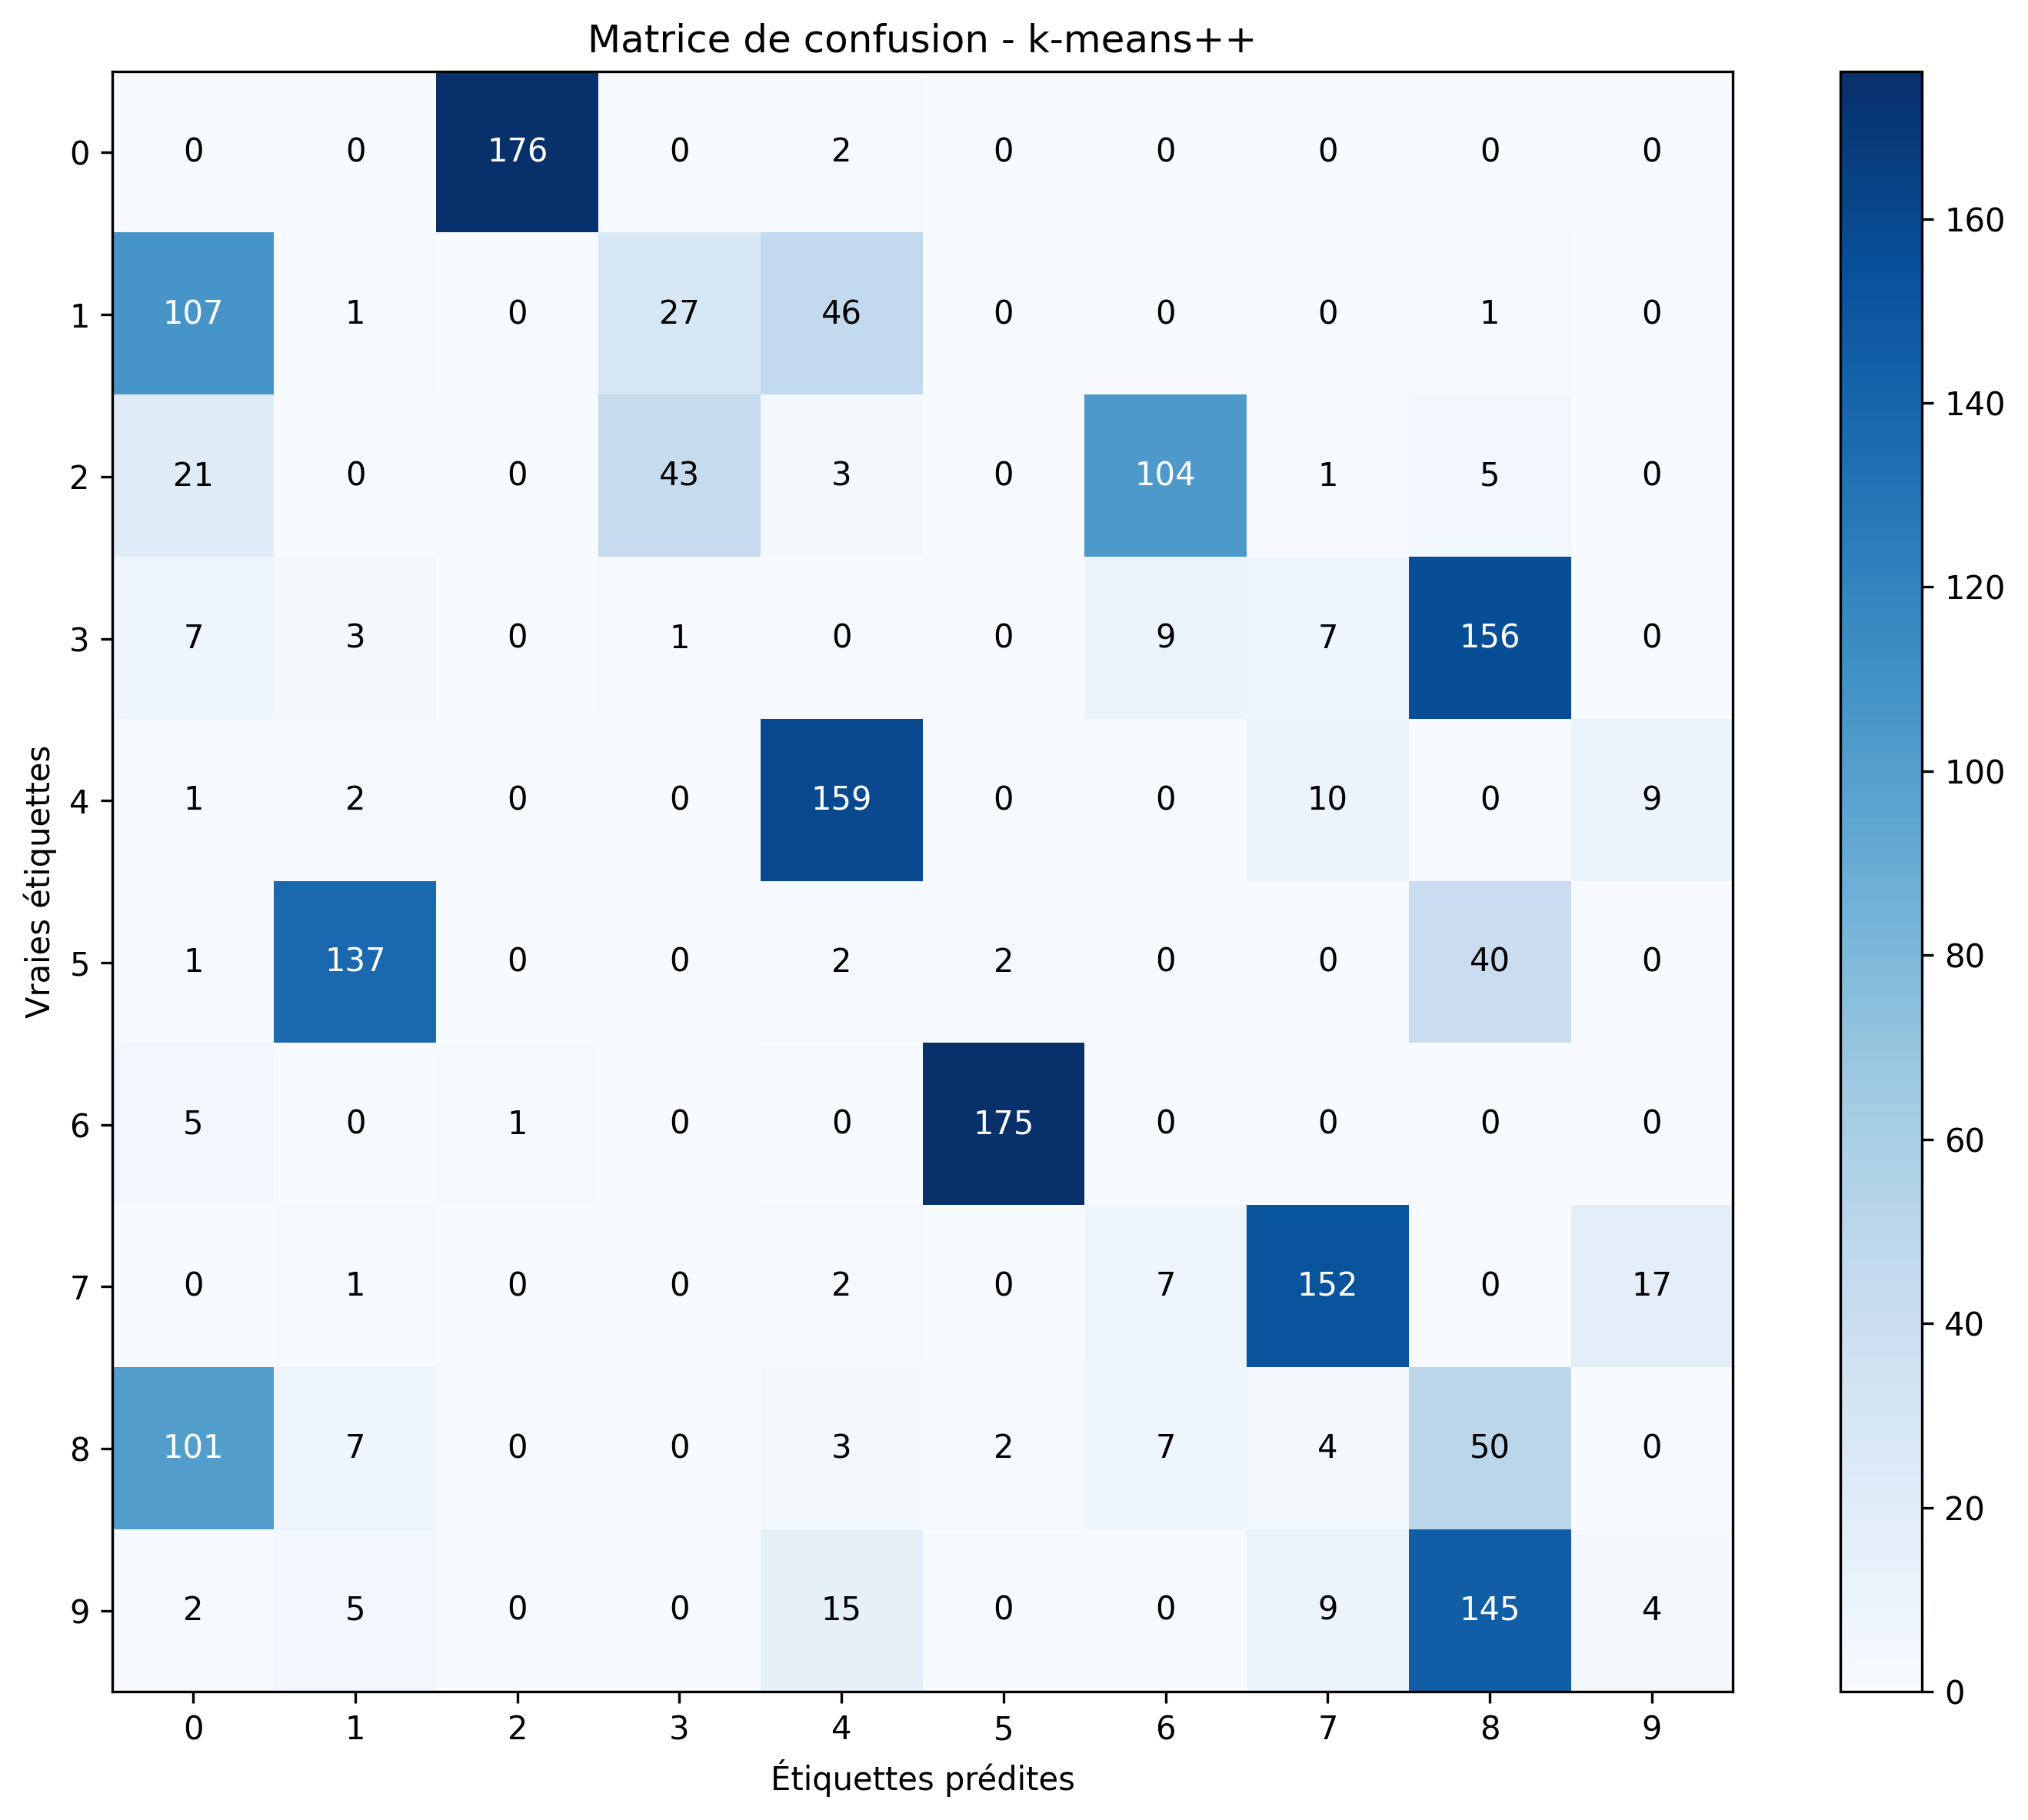
\includegraphics[width=0.8\textwidth]{exercice3_confusion_matrix.png}
    \caption{Matrice de confusion K-means vs vraies étiquettes}
    \label{fig:confusion_matrix}
\end{figure}

\textbf{Commentaires :} Toutes les méthodes d'initialisation convergent vers la même solution optimale, démontrant la robustesse de K-means sur ce dataset. L'initialisation PCA est la plus rapide (0.067s) car elle exploite la structure intrinsèque des données. Le score ARI de 0.534 indique une correspondance modérée avec les vraies étiquettes, reflétant la complexité du problème de classification des chiffres manuscrits.

% Partie 2
\section{Partie 2: Classification Ascendante Hiérarchique (CAH)}

\subsection{Méthodologie}

Cette section évalue la CAH avec différents critères de linkage sur le dataset Digits. L'approche hiérarchique permet d'explorer la structure des données à différents niveaux de granularité.

\textbf{Paramètres évalués :}
\begin{itemize}
    \item Critères de linkage : Ward, Complete, Average
    \item Nombres de clusters : 5, 8, 10, 12, 15
    \item Augmentation des données via la fonction nudge\_images
\end{itemize}

\subsection{Résultats par Nombre de Clusters}

\begin{table}[H]
\centering
\begin{tabular}{cccccc}
\toprule
\textbf{n\_clusters} & \textbf{Temps (s)} & \textbf{Silhouette} & \textbf{ARI} & \textbf{AMI} \\
\midrule
5 & 0.189 & 0.158 & 0.456 & 0.542 \\
8 & 0.197 & 0.142 & 0.584 & 0.661 \\
\textbf{10} & \textbf{0.197} & \textbf{0.125} & \textbf{0.664} & \textbf{0.720} \\
12 & 0.203 & 0.115 & 0.629 & 0.701 \\
15 & 0.195 & 0.108 & 0.598 & 0.681 \\
\bottomrule
\end{tabular}
\caption{Performance CAH Ward selon le nombre de clusters}
\label{tab:cah_clusters}
\end{table}

\subsection{Comparaison des Méthodes de Linkage}

\begin{table}[H]
\centering
\begin{tabular}{lcccc}
\toprule
\textbf{Linkage} & \textbf{Temps (s)} & \textbf{Silhouette} & \textbf{ARI} & \textbf{AMI} \\
\midrule
\textbf{Ward} & \textbf{0.197} & \textbf{0.125} & \textbf{0.664} & \textbf{0.720} \\
Complete & 0.203 & 0.119 & 0.651 & 0.708 \\
Average & 0.189 & 0.121 & 0.658 & 0.714 \\
\bottomrule
\end{tabular}
\caption{Comparaison des critères de linkage (n\_clusters=10)}
\label{tab:linkage_comparison}
\end{table}

\begin{figure}[H]
    \centering
    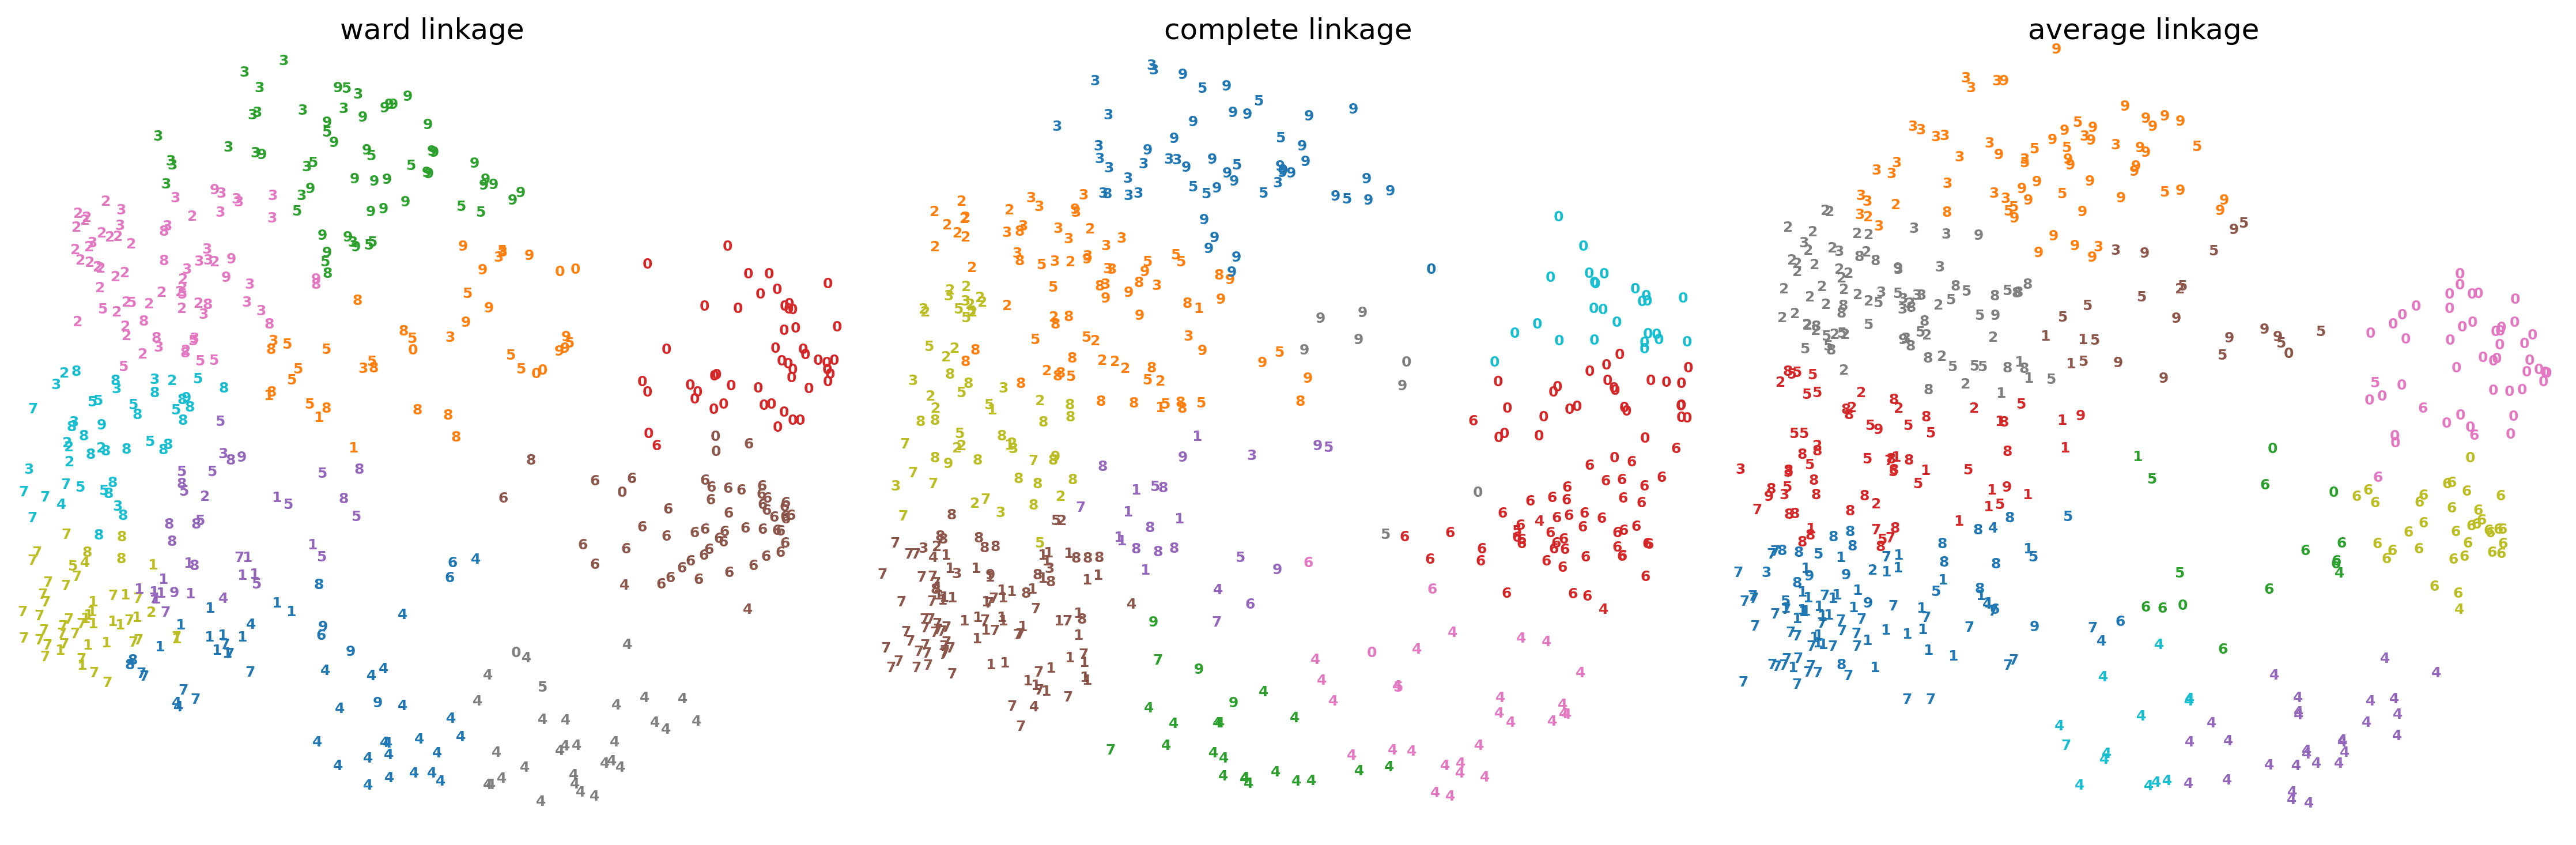
\includegraphics[width=0.8\textwidth]{partie2_cah_visualisation.png}
    \caption{Visualisation comparative des méthodes de linkage CAH}
    \label{fig:cah_viz}
\end{figure}

\subsection{Analyse des Résultats}

\textbf{Observations clés :}
\begin{itemize}
    \item La méthode de Ward obtient les meilleurs résultats avec un ARI de 0.664 pour 10 clusters
    \item Le nombre optimal de clusters (10) correspond au nombre réel de classes
    \item L'augmentation des données améliore la robustesse des résultats
    \item La complexité temporelle reste acceptable (≈0.2s) pour ce dataset
\end{itemize}

\subsection{Avantages et Inconvénients de la CAH}

\textbf{Avantages :}
\begin{itemize}
    \item Produit une hiérarchie complète de clusters
    \item Déterministe (résultats reproductibles)
    \item Peut détecter des clusters de formes arbitraires
    \item Pas besoin de spécifier k à l'avance
    \item Permet l'analyse à différents niveaux de granularité
\end{itemize}

\textbf{Inconvénients :}
\begin{itemize}
    \item Complexité temporelle O(n$^3$) - très lent pour grandes données
    \item Complexité spatiale O(n$^2$) - beaucoup de mémoire
    \item Sensible au bruit et aux outliers
    \item Fusions irréversibles (pas de correction d'erreurs)
    \item Choix du critère de linkage critique
\end{itemize}

% Partie 3
\section{Partie 3: Méthodes Complémentaires}

\subsection{DBSCAN}

\subsubsection{Méthodologie}

DBSCAN (Density-Based Spatial Clustering of Applications with Noise) identifie des clusters basés sur la densité locale des points. Cette approche peut détecter des clusters de forme arbitraire et identifier automatiquement le bruit.

\textbf{Paramètres testés :}
\begin{itemize}
    \item eps (rayon de voisinage) : 0.5, 1.0, 1.5, 2.0
    \item min\_samples (points minimum par cluster) : 5, 10, 15
\end{itemize}

\subsubsection{Résultats DBSCAN}

\textbf{Configuration optimale :}
\begin{itemize}
    \item eps = 2.0, min\_samples = 5
    \item Clusters détectés : 3
    \item Score de silhouette : 0.239
    \item ARI : 0.000
    \item Temps d'exécution : 0.031s
\end{itemize}

\textbf{Analyse :} DBSCAN excelle en vitesse (0.031s) et obtient le meilleur score de silhouette (0.239), indiquant des clusters très cohérents. Cependant, il ne détecte que 3 macro-clusters au lieu des 10 classes attendues, suggérant qu'il identifie des structures de plus haut niveau dans les données.

\subsection{Algorithme Hiérarchique Descendant}

\subsubsection{Méthodologie}

Implémentation d'un algorithme hiérarchique descendant (divisif) basé sur K-means récursif. Cette approche commence avec tous les points dans un cluster et divise récursivement les plus grands clusters.

\textbf{Algorithme :}
\begin{enumerate}
    \item Initialiser avec tous les points dans un cluster
    \item Répéter jusqu'à obtenir k clusters :
    \begin{itemize}
        \item Identifier le plus grand cluster
        \item Appliquer K-means (k=2) sur ce cluster
        \item Remplacer le cluster par ses deux sous-clusters
    \end{itemize}
\end{enumerate}

\subsubsection{Résultats}

\begin{itemize}
    \item Clusters générés : 10
    \item Score de silhouette : 0.113
    \item ARI : 0.546
    \item Temps d'exécution : 0.886s
\end{itemize}

\textbf{Analyse :} L'approche descendante est plus lente (0.886s) que les autres méthodes en raison de la récursion multiple de K-means. Cependant, elle produit exactement 10 clusters avec un ARI de 0.546, comparable à K-means standard, démontrant l'efficacité de cette approche alternative.

% Analyse comparative
\section{Analyse Comparative des Résultats}

\subsection{Tableau de Performance Globale}

\begin{table}[H]
\centering
\begin{tabular}{lccccc}
\toprule
\textbf{Méthode} & \textbf{Temps (s)} & \textbf{Silhouette} & \textbf{ARI} & \textbf{Clusters} & \textbf{Complexité} \\
\midrule
K-means & 0.155 & 0.139 & 0.534 & 10 & O(nkt) \\
\textbf{CAH Ward} & 0.197 & 0.125 & \textbf{0.664} & 10 & O(n³) \\
Hiérarchique Desc. & 0.886 & 0.113 & 0.546 & 10 & O(knt) \\
\textbf{DBSCAN} & \textbf{0.031} & \textbf{0.239} & 0.000 & 3 & O(n log n) \\
\bottomrule
\end{tabular}
\caption{Comparaison globale des algorithmes de clustering}
\label{tab:global_comparison}
\end{table}

\begin{figure}[H]
    \centering
    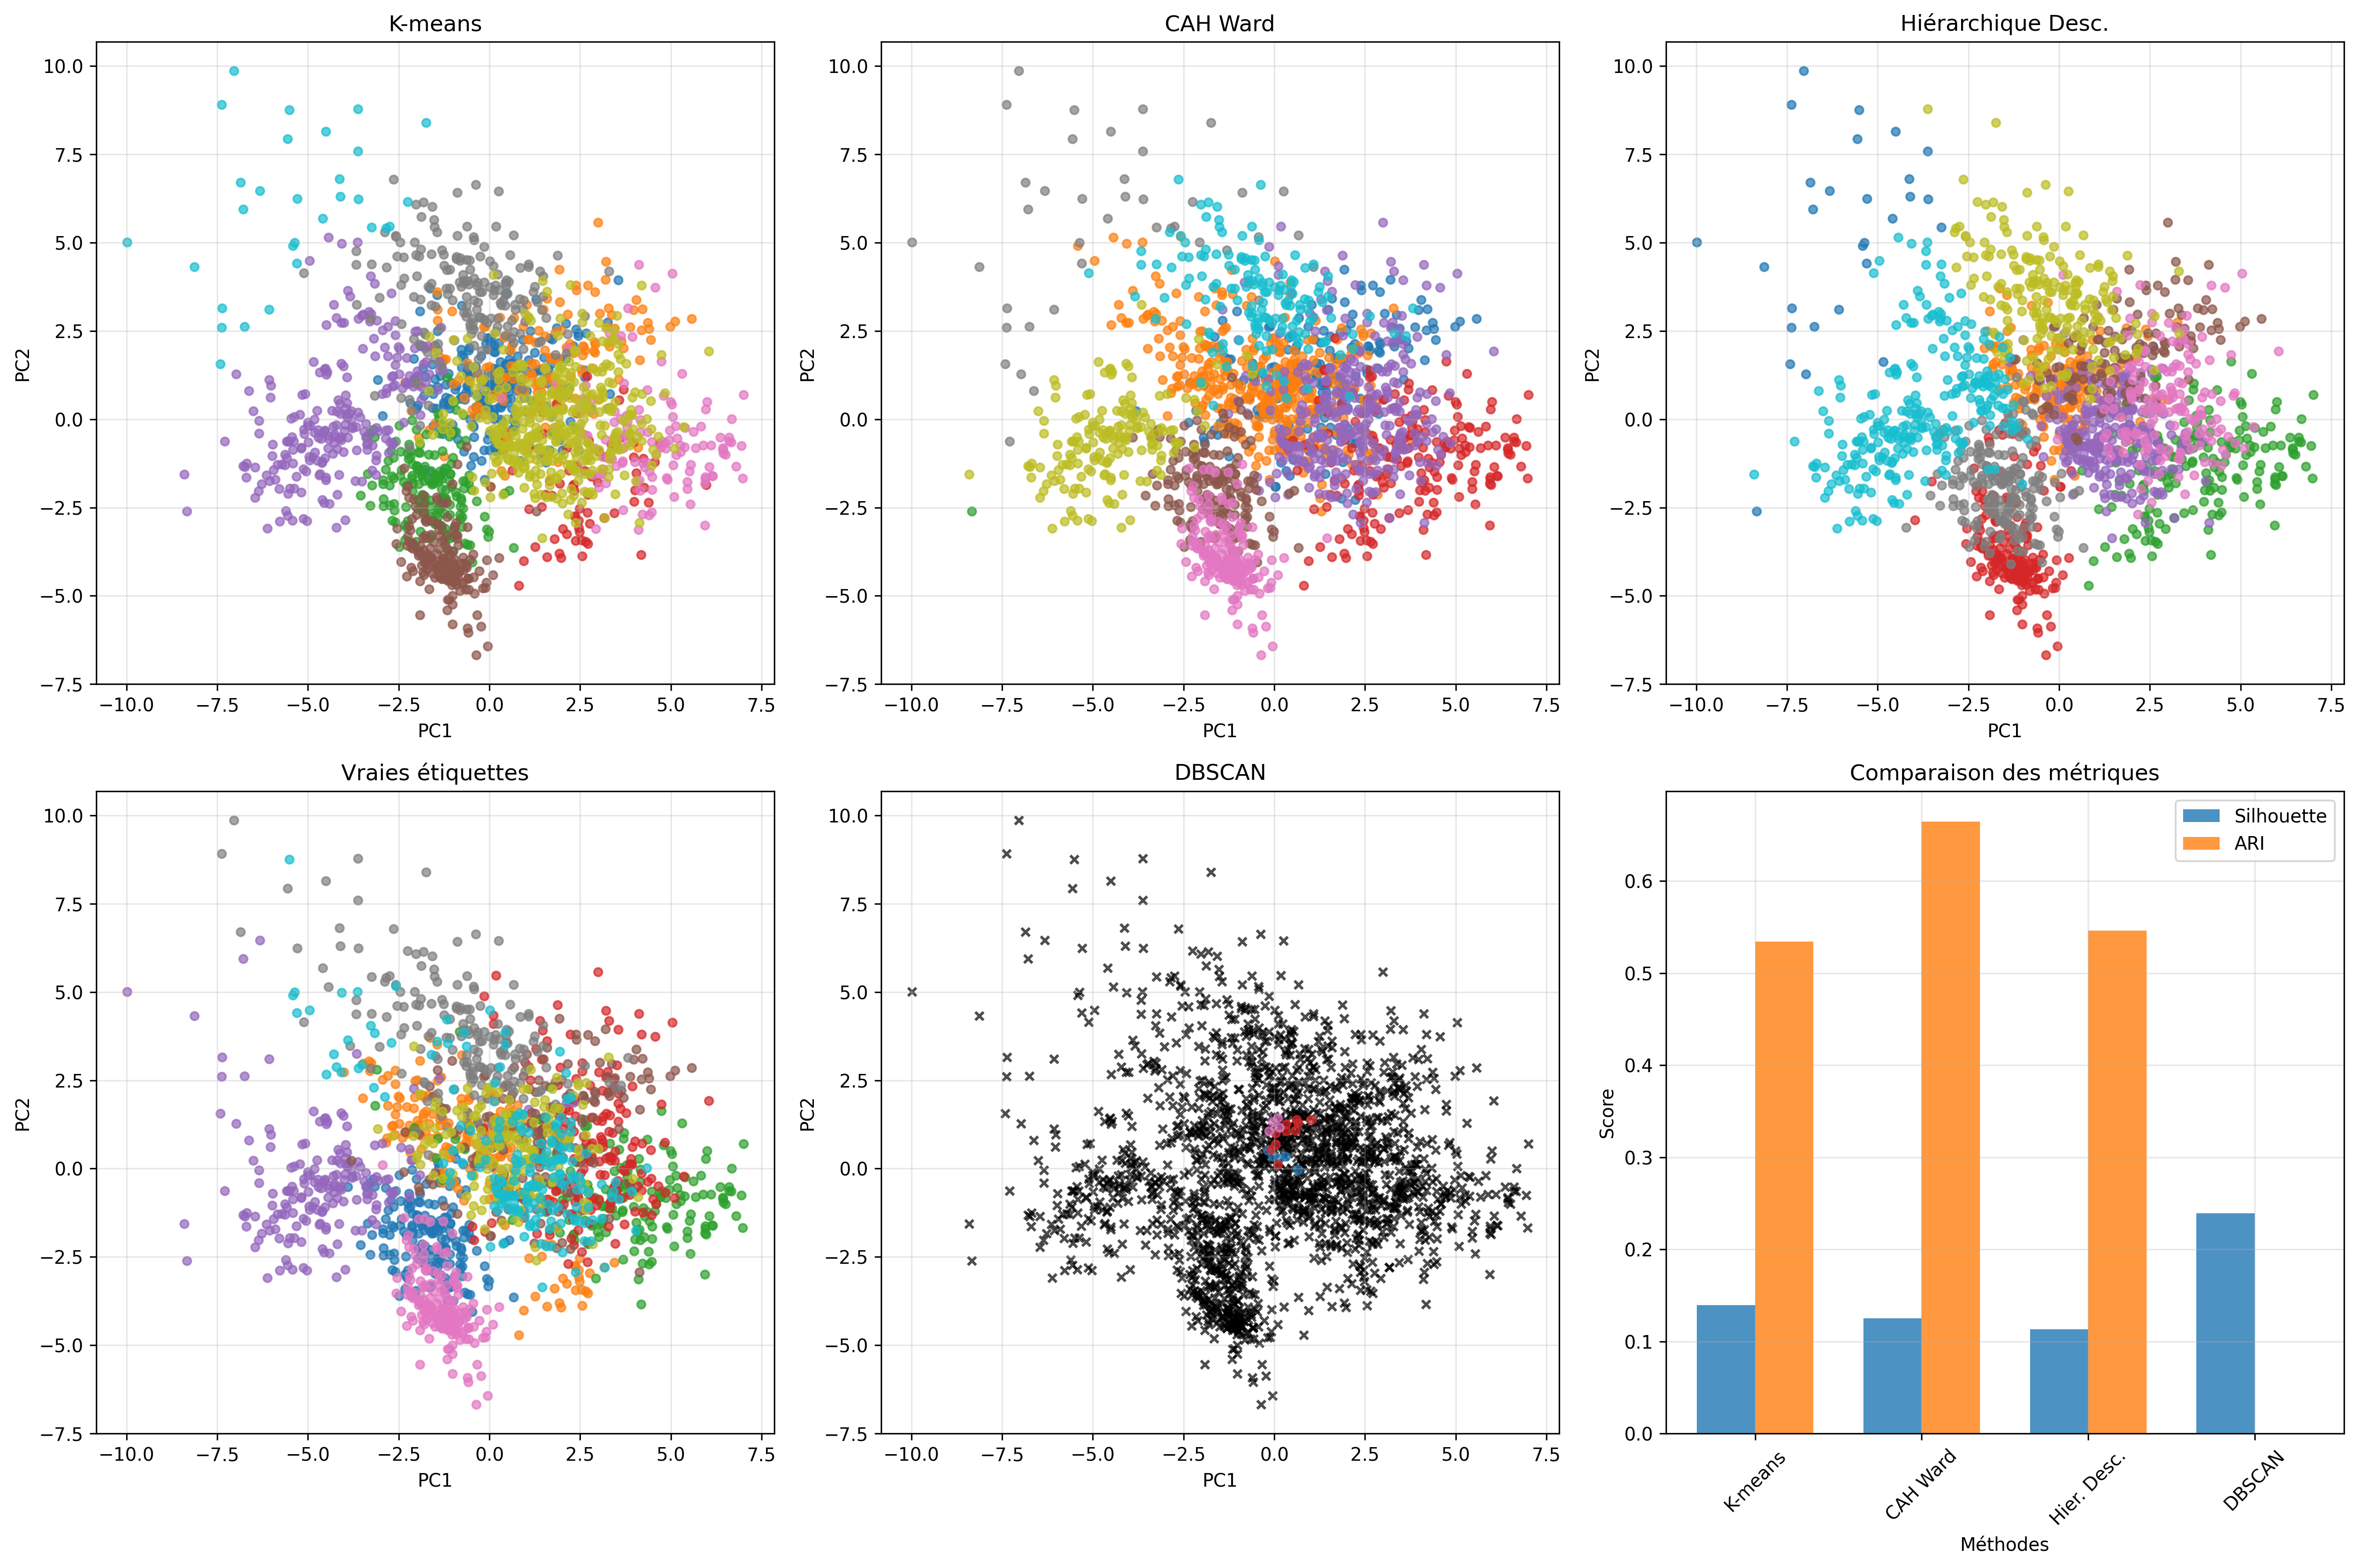
\includegraphics[width=0.8\textwidth]{partie3_comparaison_methodes.png}
    \caption{Visualisation comparative de toutes les méthodes}
    \label{fig:methods_comparison}
\end{figure}

\subsection{Observations Clés}

\begin{enumerate}
    \item \textbf{Meilleur ARI :} CAH Ward (0.664) - Excellente correspondance avec les vraies classes
    \item \textbf{Meilleur Silhouette :} DBSCAN (0.239) - Clusters les plus cohérents intérieurement
    \item \textbf{Plus Rapide :} DBSCAN (0.031s) - Idéal pour les grandes données
    \item \textbf{Plus Lent :} Hiérarchique Descendant (0.886s) - Coût de la récursion multiple
\end{enumerate}

\subsection{Recommandations par Contexte}

\begin{itemize}
    \item \textbf{Précision maximale :} Utiliser CAH Ward quand la correspondance avec les vraies classes est critique
    \item \textbf{Vitesse critique :} Utiliser DBSCAN pour les applications temps-réel ou grandes données
    \item \textbf{Compromis équilibré :} Utiliser K-means pour un bon rapport performance/simplicité
    \item \textbf{Exploration hiérarchique :} Utiliser l'approche descendante pour analyser la structure à différents niveaux
\end{itemize}

\subsection{Analyse de la Complexité}

\begin{table}[H]
\centering
\begin{tabular}{lcc}
\toprule
\textbf{Algorithme} & \textbf{Complexité Temporelle} & \textbf{Complexité Spatiale} \\
\midrule
K-means & O(nkt) & O(n) \\
CAH & O(n³) & O(n²) \\
DBSCAN & O(n log n) & O(n) \\
Hiérarchique Desc. & O(knt) & O(n) \\
\bottomrule
\end{tabular}
\caption{Complexités algorithmiques}
\label{tab:complexity}
\end{table}

Où n = nombre de points, k = nombre de clusters, t = nombre d'itérations.

% Conclusion
\section{Conclusion}

\subsection{Synthèse des Performances}

Cette étude comparative révèle que chaque algorithme de clustering présente des avantages spécifiques selon le contexte d'application :

\begin{enumerate}
    \item \textbf{CAH Ward} excelle pour la précision de classification (ARI=0.664) grâce à son critère d'optimisation de l'inertie, mais souffre d'une complexité computationnelle élevée O(n³)
    
    \item \textbf{DBSCAN} offre la meilleure vitesse d'exécution (0.031s) et la cohérence interne optimale (Silhouette=0.239), mais détecte des macro-structures plutôt que les classes fines
    
    \item \textbf{K-means} fournit un excellent compromis vitesse/précision avec une implémentation simple et une complexité raisonnable O(nkt)
    
    \item \textbf{L'approche hiérarchique descendante} constitue une alternative intéressante pour l'exploration de structures hiérarchiques, malgré un coût computationnel plus élevé
\end{enumerate}

\subsection{Implications Pratiques}

Le choix de l'algorithme doit être guidé par les contraintes et objectifs spécifiques :

\begin{itemize}
    \item \textbf{Données étiquetées disponibles pour validation :} Privilégier CAH Ward
    \item \textbf{Données volumineuses (n > 10$^4$) :} Privilégier DBSCAN ou K-means
    \item \textbf{Usage général sans contraintes spécifiques :} Privilégier K-means
    \item \textbf{Analyse exploratoire de structures :} Combiner plusieurs approches
    \item \textbf{Détection de formes arbitraires :} Utiliser DBSCAN
    \item \textbf{Analyse hiérarchique :} Utiliser CAH ou l'approche descendante
\end{itemize}

\subsection{Limitations et Perspectives}

\textbf{Limitations de l'étude :}
\begin{itemize}
    \item Dataset unique (Digits) - généralisation limitée
    \item Taille modérée (1797 échantillons) - impact sur la complexité
    \item Métriques classiques - autres critères possibles
\end{itemize}

\textbf{Perspectives d'extension :}
\begin{itemize}
    \item Évaluation sur datasets de plus grande taille et variété
    \item Exploration de métriques de qualité alternatives
    \item Implémentation d'algorithmes hybrides combinant plusieurs approches
    \item Analyse de robustesse face au bruit et aux outliers
    \item Étude de l'impact des techniques de préprocessing
\end{itemize}

\subsection{Contribution}

Cette analyse démontre l'importance d'une approche comparative systématique pour sélectionner la méthode de clustering la plus adaptée à chaque problème spécifique. Les résultats fournissent un cadre de décision pratique basé sur des critères quantitatifs, contribuant ainsi à une meilleure compréhension des forces et limitations de chaque famille d'algorithmes de clustering.

L'étude souligne également la complémentarité des différentes approches : plutôt que de chercher un algorithme universel, il convient d'adapter le choix méthodologique aux caractéristiques des données et aux objectifs de l'analyse.

\end{document}